\documentclass{beamer}

\usepackage[portuguese]{babel}
\usepackage{beamerthemeBoadilla}
%\usepackage{beamerthemeCambridgeUS}
%\usepackage{beamerthemeRochester}
%\usepackage{beamerthemeSzeged}
%\usepackage{beamerthemeMontpellier}
%\usepackage{beamerthemedefault}
\usepackage{url}
\usepackage{verbatim}
\usepackage[utf8]{inputenc}
\usepackage{multirow}

\def\Tiny{\fontsize{6pt}{6pt}\selectfont}

\title{Call Subsumption Mechanisms for Tabled Logic Programs}
\author[Flávio Cruz]{Flávio Cruz {\small \texttt{<flaviocruz@gmail.com>}}\\
Orientador: Ricardo Rocha {\small \texttt{<ricroc@dcc.fc.up.pt>}}}
\institute[CRACS]
{
  \inst{1}%
  Center for Research in Advanced Computing Systems
  \and
  \vskip-2mm
  \inst{2}%
  Faculdade de Ciências da Universidade do Porto
}
\date{\today}

\begin{document}

\frame{\titlepage}

\AtBeginSection[] { \begin{frame}<beamer>
\frametitle{Plano} \tableofcontents[currentsection]
\end{frame}}

\section{Prolog e o método SLD}

\frame
{
  \frametitle{Prolog e o método SLD}
  \begin{itemize}
     \item Na programação em lógica, o método de resolução SLD é um método inerentemente não-determinístico e do tipo \textit{top-down}.
     \item Em Prolog usa-se o método SLD de forma determinística, avaliando as cláusulas de cima para baixo e da esquerda para a direita.
     \item Esta forma de avaliação pode ser aplicado de forma eficiente em máquinas virtuais baseadas em stack, tais como a \emph{Warren's Abstract Machine} (WAM).
     \pause
     \item No entanto, este método tem diversas limitações, tais como o tratamento de ciclos infinitos (positivos ou negativos) e computações redundantes.
     
  \end{itemize}
}

\begin{frame}[fragile]
  \frametitle{Limitações do método SLD}
  \begin{columns}[t]
     \column{.5\textwidth}
     \begin{block}{Programa}
       {\small
       \begin{verbatim}
path(X, Z) :- path(X, Y),
             edge(Y, Z).
path(X, Z) :- edge(X, Z).

edge(1, 2).
edge(2, 3).
       \end{verbatim}
       }
       \begin{figure}[ht]
         \centering
           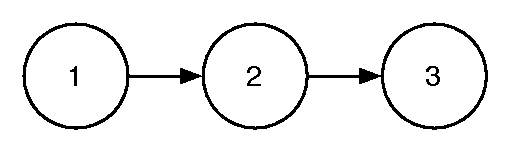
\includegraphics[scale=0.6]{edges.pdf}
       \end{figure}
     \pause
     \end{block}
      \column{.4\textwidth}
      \begin{block}{\texttt{?- path(1,~Z)}}
        \begin{figure}[ht]
          \centering
            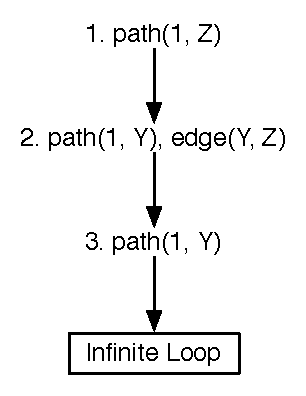
\includegraphics[scale=0.8]{inf.pdf}
        \end{figure}
      \end{block}
      
  \end{columns}
\end{frame}

\section{Tabulação}

\begin{frame}
    \frametitle{Tabulação}
    \begin{itemize}
       \item A tabulação é um refinamento do método de resolução SLD.
       \item As primeiras chamadas a subgolos tabelados são avaliados normalmente através da execução do código do
       programa.
       \item As \emph{chamadas similares} são avaliadas através do consumo das respostas guardadas na \emph{tabela}
       e que foram geradas pelo subgolo similar correspondente.
       \item Permite que programas lógicos válidos sejam executáveis.
    \end{itemize}
\end{frame}

\subsection{Similaridade de Subgolos}

\begin{frame}
   \frametitle{Similaridade entre Chamadas}
   Em geral, existem dois testes para verificar se um subgolo é similar a outro:
   \begin{itemize}
      \item \emph{Tabulação por variantes:} o subgolo $A$ é similar a $B$ quando eles são iguais por renomeação das variáveis.
      \pause
      \begin{block}{Exemplo}
         \texttt{p(X,1,Y)} e \texttt{p(Y,1,Z)} são variantes porque ambos podem ser transformados em \texttt{p(VAR0,1,VAR1)}
      \end{block}
      \pause
      \item A maioria dos motores de tabulação, incluindo o YapTab, apenas suportam este teste.
   \end{itemize}
\end{frame}

\begin{frame}
   \frametitle{Similaridade entre Chamadas}
   \begin{itemize}
   \item \emph{Tabulação por subsumpção:} $A$ é similar a $B$ quando $A$ é mais específico do que $B$ (ou $B$ é mais geral do que $A$).
   \begin{block}{Exemplo}
      \texttt{p(X,1,2)} é mais específico do que \texttt{p(Y,1,Z)} porque existe uma substituição \texttt{\{Y~=~X,~Z~=~2\}}
      que torna \texttt{p(X,1,2)} uma \emph{instância} de \texttt{p(Y,1,Z)}.
   \end{block}
   \pause
   \begin{block}{Teorema}
      Se $A$ é mais específico do que $B$ e $S_A$ e $S_B$ são os respectivos conjuntos de respostas, então $S_A \subseteq S_B$.
   \end{block}
   \pause
   \item Só o XSB Prolog implementa este tipo de tabulação, primeiro usando uma técnica chamada \textit{Dynamic Threaded Sequential Automata} (DTSA) e mais recentemente usando a técnica de \textit{Time Stamped Tries} (TST).
\end{itemize}
\end{frame}

\subsection{Exemplo}

\begin{comment}

\begin{frame}[fragile]
   \frametitle{Exemplo por variantes}
   {\tiny
   \begin{columns}[t]
         \column{.35\textwidth}
         \begin{block}{Respostas}
           {%\tiny
           \begin{itemize}
             \item<4->\alert<4>{(4) \texttt{Z = 2}}
             \item<7->\alert<7>{(7) \texttt{Z = 3}}
           \end{itemize}
           }
         \end{block}
         \column{.55\textwidth}
         \begin{block}{Programa}
           {%\tiny
             \begin{verbatim}
path(X, Z) :- path(X, Y), edge(Y, Z).
path(X, Z) :- edge(X, Z).

edge(1, 2). edge(2, 3).
               \end{verbatim}
           }
         \end{block}
     \end{columns}
     }
   \begin{block}{Exemplo}
      \begin{center}
      \includegraphics<1>[height=4.5cm]{tabled_evaluation1.pdf}%
      \includegraphics<2>[height=4.5cm]{tabled_evaluation2.pdf}%
      \includegraphics<3>[height=4.5cm]{tabled_evaluation3.pdf}%
      \includegraphics<4>[height=4.5cm]{tabled_evaluation4.pdf}%
      \includegraphics<5>[height=4.5cm]{tabled_evaluation5.pdf}%
      \includegraphics<6>[height=4.5cm]{tabled_evaluation6.pdf}%
      \includegraphics<7>[height=4.5cm]{tabled_evaluation7.pdf}%
      \includegraphics<8>[height=4.5cm]{tabled_evaluation8.pdf}%
      \includegraphics<9>[height=4.5cm]{tabled_evaluation9.pdf}%
      \includegraphics<10>[height=4.5cm]{tabled_evaluation10.pdf}%
      \includegraphics<11>[height=4.5cm]{tabled_evaluation11.pdf}%
   \end{center}
   \end{block}
\end{frame}
\end{comment}

\begin{frame}[fragile]
   \frametitle{Exemplo por Subsumpção}
   {\tiny
   \begin{columns}[t]
         \column{.55\textwidth}
         \begin{block}{Respostas}
           {%\tiny
           \begin{itemize}
              \item<1->\texttt{path(X, Z)}: \onslide<3->{\alert<3>{(3) \texttt{X=1 Z=2}}}
                     \onslide<4->{\alert<4>{(4) \texttt{X=2 Z=3}}}
                     \onslide<8->{\alert<8>{(8) \texttt{X=1 Z=3}}}
              \item<7->\texttt{path(2, Z)}: \onslide<8->{\alert<8>{(8) \texttt{Z=3}}}
              \item<9->\texttt{path(3, Z)}: \onslide<11->{$\emptyset$}
           \end{itemize}
           }
         \end{block}
         \column{.35\textwidth}
         \begin{block}{Programa}
           {%\tiny
           \begin{verbatim}
path(X, Z) :- edge(X, Z).
path(X, Z) :- edge(X, Y), path(Y, Z).

edge(1, 2). edge(2, 3).
               \end{verbatim}
           }
         \end{block}
     \end{columns}
     }
   \begin{block}{Exemplo}
      \begin{center}
      \includegraphics<1>[height=5.0cm]{sub1.pdf}%
      \includegraphics<2>[height=5cm]{sub2.pdf}%
      \includegraphics<3>[height=5cm]{sub3.pdf}%
      \includegraphics<4>[height=5cm]{sub4.pdf}%
      \includegraphics<5>[height=5cm]{sub5.pdf}%
      \includegraphics<6>[height=5cm]{sub6.pdf}%
      \includegraphics<7>[height=5cm]{sub7.pdf}%
      \includegraphics<8>[height=5cm]{sub8.pdf}%
      \includegraphics<9>[height=5cm]{sub9.pdf}%
      \includegraphics<10>[height=5cm]{sub10.pdf}%
      \includegraphics<11>[height=5.0cm]{sub11.pdf}%
   \end{center}
   \end{block}
\end{frame}

\begin{frame}
   \frametitle{Espaço das Tabelas}
   \begin{itemize}
      \item Tries: estruturas em árvore onde os prefixos comuns dos termos são representados apenas uma vez.
      \pause
      \item Normalmente, existem dois níveis de tries:
         \begin{itemize}
            \item \emph{Subgoal trie}: guarda os subgolos para um certo predicado (por exemplo \texttt{path/2}).
            \item \emph{Answer trie}: guardas as respostas.
         \end{itemize}
      \pause
   \end{itemize}
   \begin{block}{Exemplo}
     \begin{figure}[ht]
        \centering
          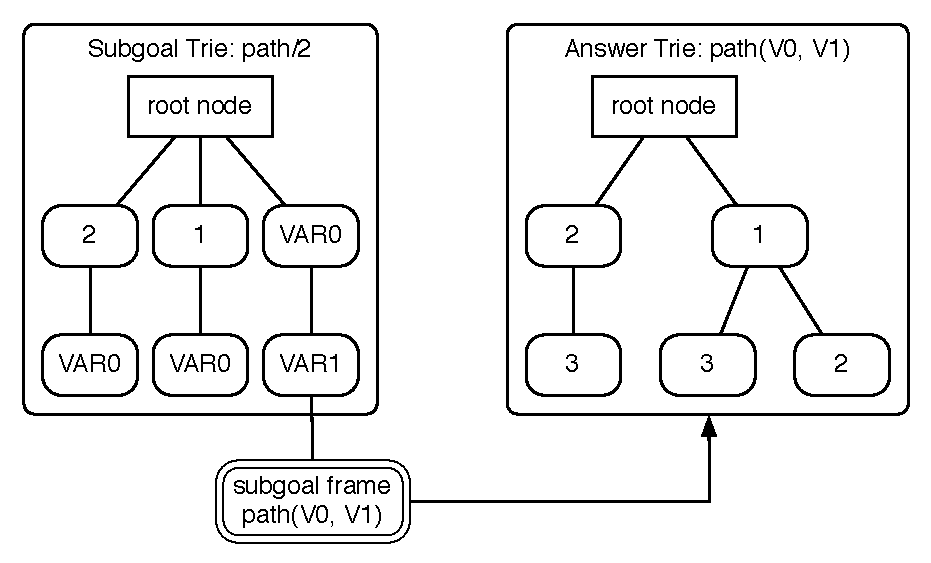
\includegraphics[scale=0.45]{two_level_tries.pdf}
      \end{figure}
    \end{block}
\end{frame}

\section{Tabulação por Subsumpção}

\begin{frame}
  \frametitle{Time Stamped Tries}
  \begin{itemize}
     \item Estende-se a answer trie com informação temporal: \emph{timestamps}.
     \item<2-> Quando uma resposta é inserida, incrementa-se o timestamp da resposta.
  \end{itemize}
  \begin{columns}[t]
        \column{.4\textwidth}
        \begin{block}{Time Stamped Trie}
          \begin{figure}[ht]
            \centering
              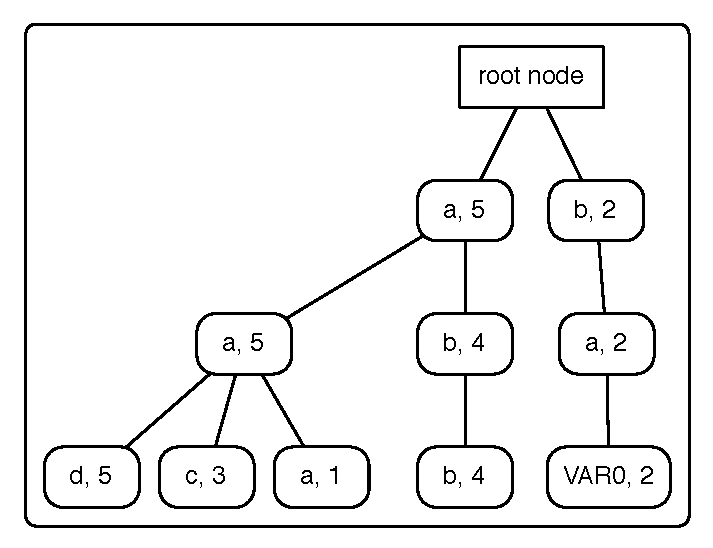
\includegraphics[scale=0.4]{tst_1.pdf}
          \end{figure}
        \end{block}
        \pause
        \column{.5\textwidth}
        \begin{block}{Inserir \textbf{p(a, b, c)}}
          \begin{figure}[ht]
            \centering
              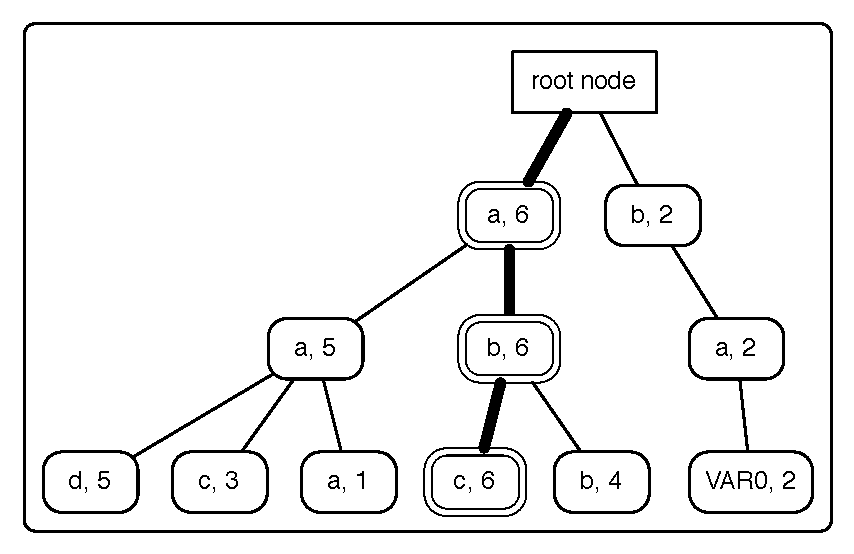
\includegraphics[scale=0.4]{tst_2.pdf}
          \end{figure}
        \end{block}
    \end{columns}
\end{frame}

\begin{frame}
  \frametitle{Time Stamped Tries}
  \begin{itemize}
     \item O subgolo específico guarda o timestamp da última procura para permitir uma pesquisa incremental.
     \item O algoritmo de pesquisa faz corte dos ramos pelo timestamp e através de operações de unificação.
  \end{itemize}
  \begin{block}{Time Stamped Trie}
      \begin{figure}[ht]
        \centering
          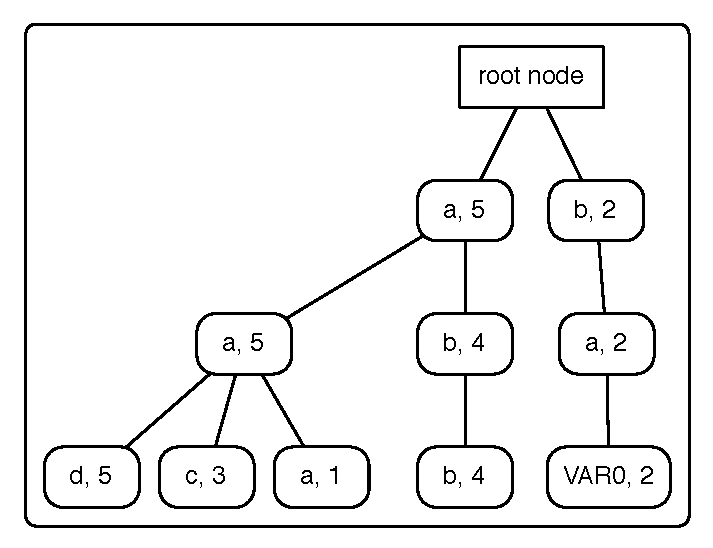
\includegraphics[scale=0.4]{tst_1.pdf}
      \end{figure}
    \end{block}
\end{frame}

\subsection{Implementação}

\begin{frame}
   \frametitle{Implementação no YapTab}
   \begin{itemize}
      \item Para implementar tabulação por subsumpção usou-se a técnica das TSTs.
      \item Reutilizou-se o código de forma quase integral do XSB Prolog: foram usados macros para
      permitir que ambos os sistemas Prolog usassem o mesmo código.
      \item As alterações nas operações principais de tabulação foram mínimas.
      \begin{itemize}
         \pause
         \item Cálculo do líder.
         \pause
         \item Nova chamada.
         \pause
         \item Nova resposta.
         \pause
         \item Calcular a próxima resposta a consumir.
         \pause
         \item Instruções da trie completa.
      \end{itemize}
      \pause
      \item \textbf{O sistema permite usar uma mistura de predicados por variantes e por subsumpção.}
   \end{itemize}
\end{frame}

\section{Tabulação por Subsumpção Retroactiva}

\subsection{Motivação}

\begin{frame}
   \frametitle{Problemas na Tabulação por Subsumpção}
   \begin{itemize}
      \item Apesar da tabulação por subsumpção atingir bons resultados, sofre de um problema:
      a ordem na qual os subgolos são chamados pode afectar a performance do sistema.
      
      \begin{block}{Exemplo}
         Se \texttt{p(1,X)} for chamado antes de \texttt{p(X,Y)}, \texttt{p(1,X)} não usará as respostas de
         \texttt{p(X,Y)}, mas irá executar o código para gerar as suas próprias respostas.
      \end{block}

   \end{itemize}
\end{frame}

\begin{frame}
   \frametitle{Como solucionar este problema?}
   \begin{itemize}
      \item Tabulação por Subsumpção Retroactiva (TSR).
      \pause
      \item Quando um subgolo $G$ é chamado, cortam-se os ramos de execução do subgolo mais
      específico $G'$ para transformar $G'$ num consumidor.
      \pause
      \item Ganhar tempo de execução e aumentar partilha de respostas.
   \end{itemize}
\end{frame}

\begin{frame}
   \frametitle{Desafios}
   \begin{itemize}
      \item Determinar que subgolos geradores e consumidores pertencem à execução do subgolo $G'$.
      \begin{itemize}
         \pause
         \item Construindo uma árvore das dependências dos subgolos.
         \pause
         \item Considerando intervalos de pontos de escolha da máquina virtual.
      \end{itemize}
      \pause
      \item Manter a execução consistente devido aos cortes.
      \begin{itemize}
         \pause
         \item Através do desenho de estratégias de controlo de execução para a resolução retroactiva.
      \end{itemize}
      \pause
      \item Evitar que o novo consumidor consuma respostas já geradas.
      \begin{itemize}
         \pause
         \item Nova organização do espaço de tabelas.
      \end{itemize}
      \pause
      \item Saber de forma eficiente que subgolos geradores mais específicos estão a executar.
      \begin{itemize}
         \pause
         \item Novo algoritmo.
      \end{itemize}
   \end{itemize}
\end{frame}

\begin{comment}
\begin{frame}[fragile]
   \frametitle{Exemplo de TSR}
   \begin{columns}[]
   \column{.35\textwidth}
   \begin{block}{Programa}
     {\tiny
     \begin{verbatim}
:- use_retroactive_tabling p/2.

a(X) :- p(1, X).

p(1, 3). p(2, 3). p(1, 2).
      \end{verbatim}
     }
   \end{block}
   \column{0.55\textwidth}
   {\small
   \begin{block}{TSR}
      \only<1>{Subgolo \texttt{p(X,Y)} é mais geral que \texttt{p(1,X)}}
      \only<2>{Subgolo \texttt{p(X,Y)} torna-se num nó retroactivo}
      \only<3>{Dado que o subgolo mais geral completou, o nó retroactivo transforma-se num nó \emph{loader}
      e carrega as soluções relevantes}
   \end{block}
   }
\end{columns}
   \begin{block}{Exemplo}
      \begin{center}
      \includegraphics<1>[height=4.5cm]{retro1.pdf}%
      \includegraphics<2>[height=4.5cm]{retro2.pdf}%
      \includegraphics<3>[height=4.5cm]{retro3.pdf}%
   \end{center}
   \end{block}
\end{frame}
\end{comment}


\begin{frame}[fragile]
   \frametitle{Exemplo de Execução}
   \begin{columns}[]
   \column{.35\textwidth}
   \begin{block}{Programa}
     {\Tiny
     \begin{verbatim}
:- use_variant_tabling [a/2, b/1].
:- use_retroactive_tabling p/2.

a(X, Y) :- p(1, X), b(Y).
a(3, 4).
b(1). b(2).
p(1, X) :- a(_, X).
p(1, X) :- b(X).
      \end{verbatim}
     }
   \end{block}
   \column{0.55\textwidth}
   {\small
   \begin{block}{TSR}
      \only<1>{Novo gerador \texttt{a(X,Y)}}
      \only<2>{Novo gerador \texttt{p(1,X)}}
      \only<3>{Novo consumidor \texttt{a(\_,X)}}
      \only<4>{Novo gerador \texttt{b(X)}}
      \only<5>{Novo consumidor \texttt{b(Y)}}
      \only<6>{Novo gerador mais geral \texttt{p(Z,W)}}
      \only<7>{Determinar ramos a cortar}
      \only<8>{Consumidores como o \texttt{a(\_,X)} são simplesmente removidos do \emph{dependency space}}
      \only<9>{\texttt{b(X)} é um subgolo gerador interno, mudar o seu estado para \emph{pruned}.
      Transformar \emph{consumidores externos} (\emph{orphaned consumers}) em nós retroactivos}
      \only<10>{O nó \texttt{b(Y)} é um \emph{nó fronteira}. É necessário ligá-lo ao nó \texttt{p(1,X)} para
      evitar que a execução salte para ramos mortos}
      \only<11>{Transformar o nó \texttt{p(1,X)} em nó retroactivo e remover o \emph{subgoal frame} da
      pilha respectiva}
      %\only<12>{Novo consumidor \texttt{a(\_,W)}}
      %\only<13>{Gerador \texttt{b(V0)} é reactivado e completa}
      %\only<14>{Subgolo \texttt{p(Z,W)} tenta completar mas não é líder}
      %\only<15>{Após backtracking, o nó retroactivo \texttt{b(Y)} executa a instrução de resolução retroactiva
      %e transforma-se num nó carregador (\emph{loader})}
      %\only<16>{Ao chegar-mos ao nó \texttt{p(1,X)}, este é transformado num consumidor, pois \texttt{p(Z,W)}
      %ainda não completou}
      %\only<17>{O subgolo \texttt{a(X,Y)} como líder poderá depois completar a computação em segurança}
   \end{block}
   }
\end{columns}
   \begin{block}{Exemplo}
      \begin{center}
         \includegraphics<1>[height=4.1cm]{issues1.pdf}%
         \includegraphics<2>[height=4.1cm]{issues2.pdf}%
         \includegraphics<3>[height=4.1cm]{issues3.pdf}%
         \includegraphics<4>[height=4.1cm]{issues4.pdf}%
         \includegraphics<5>[height=4.1cm]{issues5.pdf}%
         \includegraphics<6>[height=4.1cm]{issues6.pdf}%
         \includegraphics<7>[height=4.1cm]{issues7.pdf}%
         \includegraphics<8>[height=4.1cm]{issues8.pdf}%
         \includegraphics<9>[height=4.1cm]{issues9.pdf}
         \includegraphics<10>[height=4.1cm]{issues10.pdf}
         \includegraphics<11>[height=4.1cm]{issues11.pdf}
         %\includegraphics<12>[height=4.1cm]{issues12.pdf}
         %\includegraphics<13>[height=4.1cm]{issues13.pdf}
         %\includegraphics<14>[height=4.1cm]{issues14.pdf}
         %\includegraphics<15>[height=4.1cm]{issues15.pdf}
         %\includegraphics<16>[height=4.1cm]{issues16.pdf}
         %\includegraphics<17>[height=4.1cm]{issues17.pdf}
      \end{center}
   \end{block}
\end{frame}

\subsection{Corte da Execução}

\begin{frame}
   \frametitle{Corte da Execução}
   \begin{itemize}
      \item Existem dois tipos de corte dependendo onde o subgolo mais geral aparece relativamente ao subgolo específico:
      \begin{itemize}
         \item Corte externo: se aparece fora (visto anteriormente).
         \pause
         \item Corte interno: se aparece dentro.
      \end{itemize}
      \pause
      \item Independente do tipo de corte, existe um conjunto de problemas que advém do corte da execução
      de geradores ou consumidores internos ao subgolo específico:
      \begin{itemize}
         \item \emph{Orphaned Consumers} (visto anteriormente)
         \pause
         \item \emph{Lost consumers}
         \pause
         \item \emph{Pseudo-Completion}
         \pause
         \item \emph{Leader Re-Computation}
      \end{itemize}
   \end{itemize}
\end{frame}

\begin{frame}
   \frametitle{Corte Interno}
   \begin{itemize}
      \item Nesta situação cortam-se os ramos referentes a $G'$, excepto a parte que irá
      computar as soluções do subgolo $G$.
      \begin{itemize}
         \item $G$ executa normalmente mas não devolve as soluções para o ambiente externo\footnote{O subgolo
         executa usando \emph{local scheduling}}.
      \end{itemize}
      \item<2-> Quando $G$ ou completar ou não conseguir completar por ser o líder, salta-se para o ponto
      de escolha do subgolo $G'$.
   \end{itemize}
   \begin{columns}[t]
         \column{.45\textwidth}
         \begin{block}{Antes}
           \begin{figure}[ht]
             \centering
               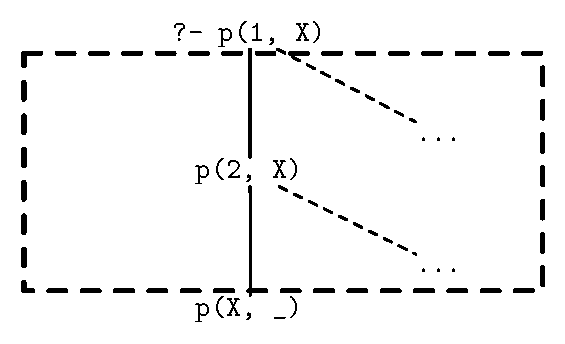
\includegraphics[scale=0.4]{internal1.pdf}
           \end{figure}
         \end{block}
         \pause
         \column{.45\textwidth}
         \begin{block}{Depois}
           \begin{figure}[ht]
             \centering
               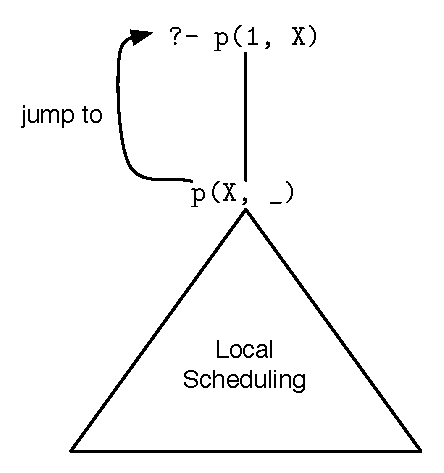
\includegraphics[scale=0.30]{internal2.pdf}
           \end{figure}
         \end{block}
     \end{columns}
\end{frame}

\subsection{Espaço das Tabelas}
\begin{frame}
   \frametitle{Espaço das Tabelas}
   \begin{itemize}
      \item \emph{Single Time Stamped Trie}: uma \emph{answer trie} única por predicado.
      \begin{itemize}
         \item As respostas são representadas apenas uma vez e referenciadas pelos subgolos que as usam.
         \item Usa-se um timestamp por cada subgolo de forma a facilitar a transformação de gerador para consumidor.
      \end{itemize}
      \item<2-> Permite que se possam reutilizar respostas relevantes a um novo subgolo gerador antes de executar
      o código.
   \end{itemize}
   \begin{block}{Single Time Stamped Trie}
     \begin{figure}[ht]
       \centering
         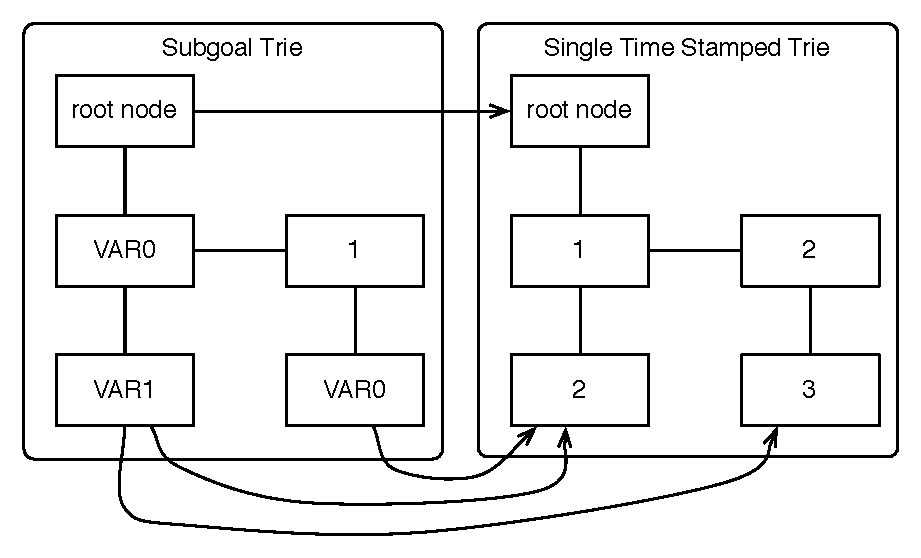
\includegraphics[scale=0.37]{stst.pdf}
     \end{figure}
   \end{block}
\end{frame}

\subsection{Procura de Subgolos Específicos}
\begin{frame}
   \frametitle{Procura de Subgolos Específicos}
   \begin{itemize}
      \item Percorrer a \emph{subgoal trie} para encontrar subgolos mais específicos.
      \pause
      \item O problema resume-se a encontrar atribuições para as variáveis do subgolo mais geral.
      \item Usa-se a heap e a trilha da máquina virtual para maior eficiência.
      \pause
      \item Para melhorar a eficiência, estendeu-se cada nó da \emph{subgoal trie} com o número de
      subgolos sobre aquele ramo da trie que estão a executar.
   \end{itemize}
   \begin{columns}[t]
        \column{.45\textwidth}
        \begin{block}{Subgoal trie}
          \begin{figure}[ht]
            \centering
              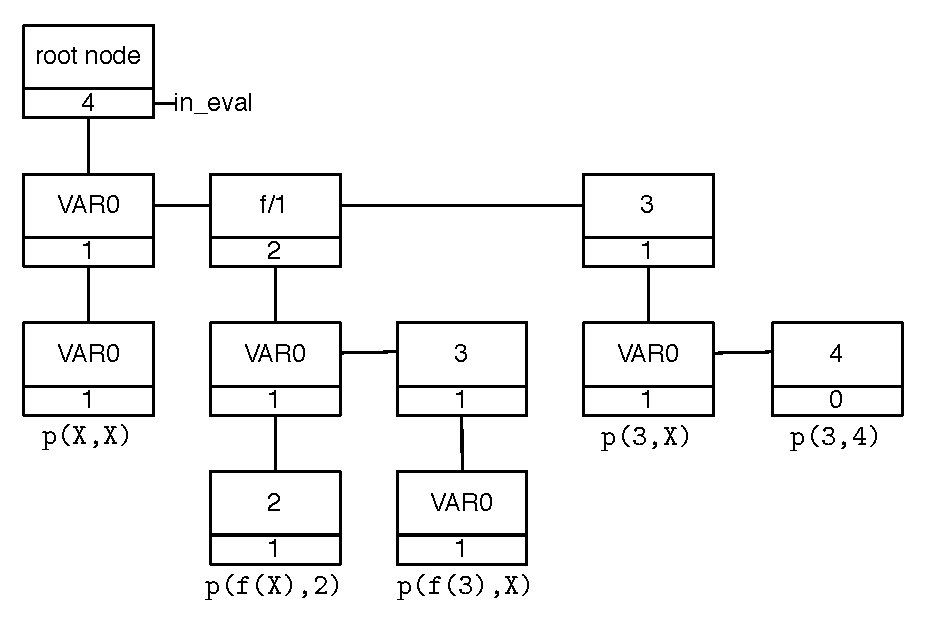
\includegraphics[scale=0.31]{in_eval_trie.pdf}
          \end{figure}
        \end{block}
         \column{.45\textwidth}
         \begin{block}{Novo gerador}
           \begin{figure}[ht]
             \centering
               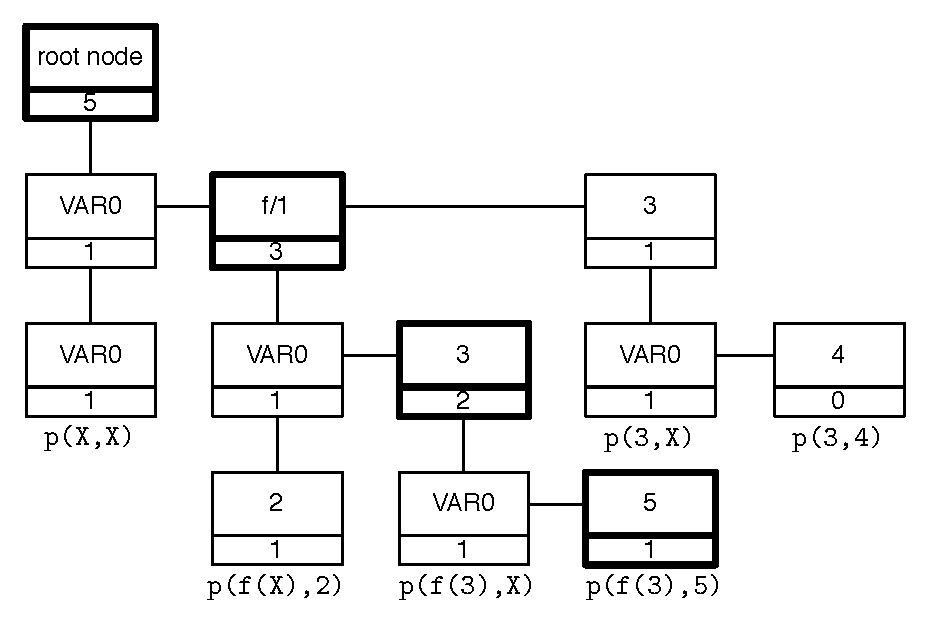
\includegraphics[scale=0.31]{in_eval_add.pdf}
           \end{figure}
         \end{block}

     \end{columns}
\end{frame}

\section{Resultados}

\begin{frame}
   \frametitle{Tabulação por Subsumpção}
   \begin{itemize}
      \item Avaliou-se o desempenho do motor de tabulação por subsumpção e comparou-se com
      o motor de tabulação do XSB Prolog.
      \item Sendo que ambos usam os mesmos algoritmos e estruturas de dados, o desempenho é muito
      parecido.
   \end{itemize}
   {\footnotesize
   \begin{center}
     \begin{tabular}{ccc}
      \hline
       \hline
       \multirow{2}{*}{\textbf{Programa}} & \textbf{XSB Prolog} & \textbf{Yap Prolog} \\
       & \textit{\small{Speedup médio}} & \textit{\small{Speedup médio}} \\
      \hline
      \hline
   left\_first & 0.78 & \textbf{1.02} \\
   left\_last & 0.77  & \textbf{0.96} \\
   right\_first & \textbf{1.01} & \textbf{1.01} \\
   right\_last & 0.94 & \textbf{1.07} \\
   double\_first & 1.37 & \textbf{1.48} \\
   double\_last & 1.31 & \textbf{1.40} \\
   samegen & \textbf{339.76} & 1.03 \\
   genome & 559.54 & \textbf{648.51} \\
   reach\_first  & \textbf{0.96} & 0.94 \\
   reach\_last  & \textbf{0.97} & 0.90 \\
   \hline
   \hline
   \end{tabular}
   \end{center}}
\end{frame}

\begin{frame}
   \frametitle{Custo da TSR}
   \begin{itemize}
      \item Foi medido o desempenho da TSR para programas que não tiram vantagens de usar os novos
      mecanismos.
      \item Comparou-se o desempenho com tabulação por subsumpção tradicional e tabulação por variantes.
   \end{itemize}
   \begin{center}
      {\footnotesize
     \begin{tabular}{ccc}
      \hline
       \hline
       \multirow{2}{*}{\textbf{Programa}} & \multicolumn{2}{c}{\textbf{Yap Prolog}} \\
       & \textit{\small{Retro / Var}} & \textit{\small{Retro / Sub}} \\
      \hline
      \hline
      left\_first & 1.06 & 1.01 \\
      left\_last &  1.07  & 1.03 \\
      right\_first & \textbf{0.97} & \textbf{0.95} \\
      right\_last & 1.25 & \textbf{0.94} \\
      double\_first & 1.01 & 1.16 \\
      double\_last & 1.04 & 1.16 \\
      samegen & 1.19 & 1.14 \\
      reach\_first  &  1.11  & 1.04 \\
      reach\_last  &  1.17  & 1.04 \\
   \hline
   \hline
   \textit{Média Total} &  1.10 &  1.05 \\
   \hline
   \hline
   \end{tabular}}
\end{center}
\end{frame}

\begin{frame}
   \frametitle{Ganhos da TSR}
   
   \begin{itemize}
      \item Por outro lado, comparou-se o desempenho para programas onde usar TSR é vantajoso.
   \end{itemize}
   \begin{center}
   {\footnotesize
     \begin{tabular}{ccc}
      \hline
       \hline
       \multirow{2}{*}{\textbf{Programa}} & \multicolumn{2}{c}{\textbf{Yap Prolog}} \\
       & \textit{\small{Var / Retro}} & \textit{\small{Sub / Retro}} \\
      \hline
      \hline
   left\_first\footnote{Para os programas do tipo \texttt{path/2} usou-se o golo \texttt{path(X,1)}.} & 0.89 & 0.95 \\
   left\_last & 0.88  & 0.90 \\
   double\_first & 1.07 & \textbf{1.09} \\
   double\_last & 1.05 & \textbf{1.10} \\
   genome & 450.33 & 0.74 \\
   reach\_first  & 2.54 & \textbf{1.76} \\
   reach\_last  & 3.22 & \textbf{1.87} \\
   flora & 3.17 & \textbf{1.17} \\
   fib & 1.95 & \textbf{2.02} \\
   big & 13.26 & \textbf{13.66} \\
   \hline
   \hline
   \end{tabular}}
   \end{center}
\end{frame}

\section{Conclusões}

\begin{frame}
   \frametitle{Conclusões}
   \begin{itemize}
      \item Contribuições:
      \begin{itemize}
         \item YapTab suporta tabulação por subsumpção.
         \item Mecanismos e algoritmos que controlam a execução retroactiva.
         \item Algoritmo de pesquisa de subgolos específicos.
         \item Espaço de tabelas inovador que permite uma maior reutilização de respostas.
         \item Suporte para uma mistura de métodos de avaliação: retroactivo, variantes e subsumpção.
         \pause
      \end{itemize}
      \item Trabalho futuro:
      \begin{itemize}
         \item Integrar o trabalho na distribuição oficial do Yap Prolog.
         \item Melhoramento dos algoritmos do espaço das tabelas.
         \item Maior experimentação com aplicações reais.
         \item Explorar outros métodos de avaliação, como o \emph{Call Abstraction}.
      \end{itemize}
   \end{itemize}
\end{frame}

\begin{frame}
   \frametitle{Artigos Publicados}
   \begin{itemize}
      \item Retroactive Subsumption-Based Tabled Evaluation of Logic Programs, Flávio Cruz and Ricardo Rocha. 12th European Conference on Logics in Artificial Intelligence (JELIA 2010), Springer-Verlag. Helsinki, Finland, September 2010.
      \item Submetidos:
         \begin{itemize}
      \item Efficient Instance Retrieval of Executing Subgoals for Tabled Evaluation, Flávio and Ricardo Rocha. 17th International Conference on Logic for Programming, Artificial Intelligence and Reasoning (LPAR 17), Yogyakarta, Indonesia, October 2010.
      \item Efficient Retrieval of Subsumed Subgoals in Tabled Logic Programs, Flávio Cruz and Ricardo Rocha. Compilers, Programming Languages, Related Technologies and Applications (CORTA 2010), Braga, Portugal, September 2010.
   \end{itemize}
   \end{itemize}
\end{frame}
   
\end{document}